\documentclass[a4paper,11pt]{article}
\usepackage{makeidx}
\usepackage{url}
\usepackage{graphicx}
\usepackage{amsmath}
\usepackage{amssymb}
\usepackage{color}
%\usepackage{ifthen}
\usepackage{array}
%\usepackage{wrapfig}
%\usepackage{multirow}
\usepackage{cite}


\title{\textbf{Adding the trapezoidal rule as an option to the EulerImplicitSolver in Sofa}}
\author{D. John, H. Talbot}
\date{14.12.2015}

\begin{document}

\maketitle

\section{Mathematical problem}
The equation we would like to solve is
\begin{align} 
M \dot{y}(t) = f(y(t)),\quad  y(0) = y_0, 
\end{align}
and implicitly formulated for $t_{n+1} = t_{n} + h $ it is 
\begin{align} \label{ode}
M \dot{y}_{n+1} = f(y_{n+1}),
\end{align}
where $y_{n+1} = y(t_{n+1})$.



\subsection*{Implicit Euler}
% The most used time integration scheme in Sofa is the implicit Euler scheme. 
Here, we briefly present the well known implicit Euler method and how it is implemented in Sofa.
For ordinary differential equations (ODE's) of first order 
\begin{align*}
\dot{y}(t) &= f (t,y(t)), \quad \text{for } t>0,\\
y(0) &= y_0,
\end{align*}
the implicit Euler scheme states 
\begin{align}
y_{n+1} - y_{n} = h f(y_{n+1}).
\end{align}
For this method Taylor's expansion and the chain rule are used for equation~\eqref{ode}
\begin{align*}
M \dot{y}_{n+1} &= f(y_{n}) + h \dot{f}(y_{n+1}), \\
M \dot{y}_{n+1} &= f(y_{n}) + h \dfrac{\partial f}{\partial x} \dot{y}_{n+1},
\end{align*}
resulting in the system of linear equations
\begin{align*}
\left( M -h K \right) \dot{y}_{n+1} &= f(y_{n}).
\end{align*}
Solving this we get the velocity $\dot{y}_{n+1}$ and are able to compute the new positions $y_{n+1}$ with
\begin{align*}
y_{n+1} = y_{n} + h \dot{y}_{n+1}.
\end{align*}


The implicit Euler method for second order ODE's is based on following equations
\begin{align*}
{y}_{n+1} &= {y}_{n} + h \dot{y}_{n+1}, \\
\dot{y}_{n+1} &= \dot{y}_{n} + h \ddot{y}_{n+1}.
\end{align*}
The unknown is
\begin{align*}
\Delta \dot{y} := \dot{y}_{n+1} - \dot{y}_{n}.
\end{align*}
We obtain for the system of linear equations 
\begin{align*}
M \Delta\dot{y} &= h f(y_{n+1}), \\
M \Delta\dot{y} &= h \left( f(y_{n}) +  h K (\dot{y}_{n} + \Delta\dot{y}) + (B - r_M M +r_K K)  (\dot{y}_{n} + \Delta\dot{y}) \right),
\end{align*}
where
\begin{align*}
M& \ \text{ is the mass matrix},\\
K& = \dfrac{\partial f}{\partial y} \text{ is the stiffness matrix and}\\
B& = \dfrac{\partial f}{\partial \dot{y}} \text{ is the damping}.
\end{align*}
Hence we need to solve
\begin{align*}
\left( (1+h r_M) M - h B - h (h+r_K) K \right) \Delta\dot{y} &= h \left( f(y_{n}) +  ((h+r_K) K + B - r_M M) \dot{y}_{n} \right).
\end{align*}
The implicit Euler method is of first order accuracy and A-stable. 

% TODO Add projection matrix


\subsection*{Trapezoidal rule}
In the following we will briefly present the well known trapezoidal rule and how it is added as an option to the already existing EulerImplicitSolver in Sofa.
The advantage of the trapezoidal rule is that it has second order accuracy by containing A-stability.

The trapezoidal rule for first order ODE's is based on following scheme
\begin{align*}
y_{n+1} - y_{n} = \dfrac{h}{2} \left( f(y_{n+1}) + f(y_{n}) \right)
\end{align*}
With the same expansion of $f(y_{n+1})$ as in the derivation of the implicit Euler scheme we receive  for a first order differential equation
\begin{align*}
\left( M - \dfrac{h}{2} K \right) \dot{y}_{n+1} &= f(y_{n})
\end{align*}
and for a second order differential equation 
\begin{align*}
\left( (1+ \frac{h}{2} r_M) M - \frac{h}{2} B - \frac{h}{2} (h+r_K) K \right) \Delta\dot{y} &= \frac{h}{2} \left( 2 f(y_{n}) +  ((h+r_K) K + B - r_M M) \dot{y}_{n} \right).
\end{align*}
Since the differences to the implicit Euler method are very small (just a few factors) it can easily be implemented as a second order option for the already in Sofa existing EulerImplicitSolver. The trapezoidal rule can be activated by setting the option trapezoidalScheme = 'true'.


% Since it is important for medical simulations to simulate in real time we need to compare the cost of the trapezoidal rule to the implicit Euler scheme. (no. of CG iterations, computing time, \dots) 



\subsection{Mechanical example}
As a mechanical example with a analytical solution we consider a spring mass pendulum.
The equation of motion is
\begin{align*}
\ddot{x}(t) &= \frac{K_s}{m} x(t),\\
\dot{x}(0) &= 0,\\
x(0) &= A,
\end{align*}
where $x(t)$ is the position of the mass $m$, $K_s$ is the stiffness of the spring and $A = g \frac{m}{K_s}$ the amplitude of the motion with $g$ the gravitation.
The analytical solution is
\begin{align*}
x(t) = A \cos(\sqrt{({K_s}/{m})} \ t).
\end{align*}

%TODO: add sketch

We set the length of the spring $l=1$, $m=1$, $K_s = 100$, $g=10$ and hence $A = 0.1$.
By creating a scene and simulate with Sofa we received the results depicted in figure \ref{fig1}, where the error is the absolute error compared to the analytical solution. 
This clearly shows an improvement in accuracy. 

\begin{figure}[ht]
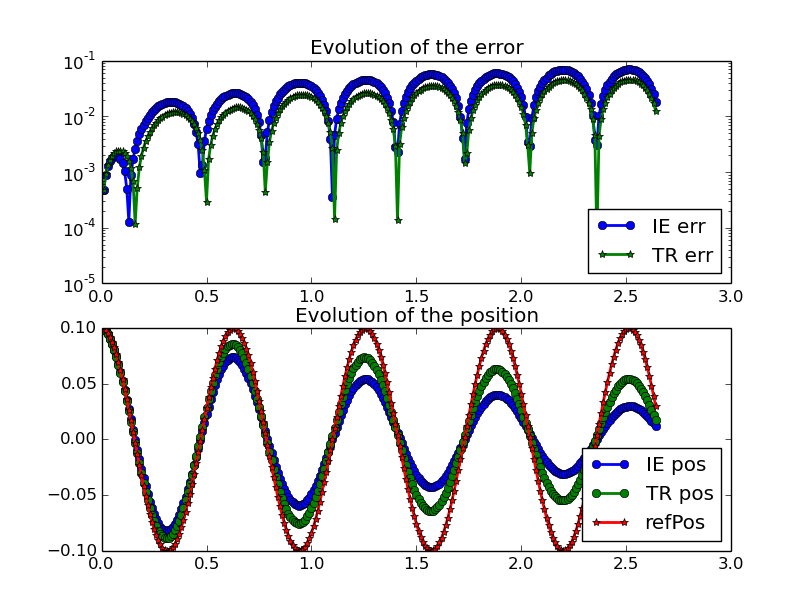
\includegraphics[scale= 0.75]{fig_impliciteuler_trapezoidal_dt0_01_spring.png}
\caption{Error and position for solving the spring mass pendulum in Sofa by implicit Euler and trapezoidal rule for $h = 0.01$.}
\label{fig1}
\end{figure}





\end{document}



